\chapter{Системийн архитектур, зохиомж}

\section{Системийн архитектур}

Cистемийн архитектур нь дараах хүчин зүйлсээс шалтгаална.

\begin{enumerate}
	\item Хэрэв олон тооны хэрэглэгчдийг хүлээж байгаа бол томрох боломжтой архитектурыг сонгох хэрэгтэй бөгөөд ингэснээр илүү их урсгалыг зохицуулахын тулд илүү олон сервер нэмж болно.
	\item Cистем үргэлж бэлэн байх өндөр хүртээмжтэй архитектурыг сонгох хэрэгтэй бөгөөд энэ нь зарим бүрэлдэхүүн хэсэг нь бүтэлгүйтсэн ч үргэлжлүүлэн ажиллах боломжтой.
	\item Хэрэглэгчийн мэдрэмтгий өгөгдлийг хадгалдаг бол аюулгүй, халдлагыг тэсвэрлэх чадвартай архитектурыг сонгох хэрэгтэй.
\end{enumerate}

Даараах хүчин зүйлсүүдийг хамааран (Three-tier) үлгэр загварыг сонголоо. Вэб системийн нийтлэг архитектур бөгөөд танилцуулгын түвшин, хэрэглээний түвшин, мэдээллийн баазын түвшин гэсэн гурван давхаргаас бүрдэнэ. Үзүүлэнгийн түвшин нь хэрэглэгчийн интерфэйсийг зохицуулж, үр дүнг хэрэглэгчдэд харуулдаг. Хэрэглээний давхарга нь системийн логикийг зохицуулж, мэдээллийн сантай харьцдаг. Өгөгдлийн сангийн давхарга нь системийн өгөгдлийг хадгалдаг.

\begin{figure}[h]
	\centering
	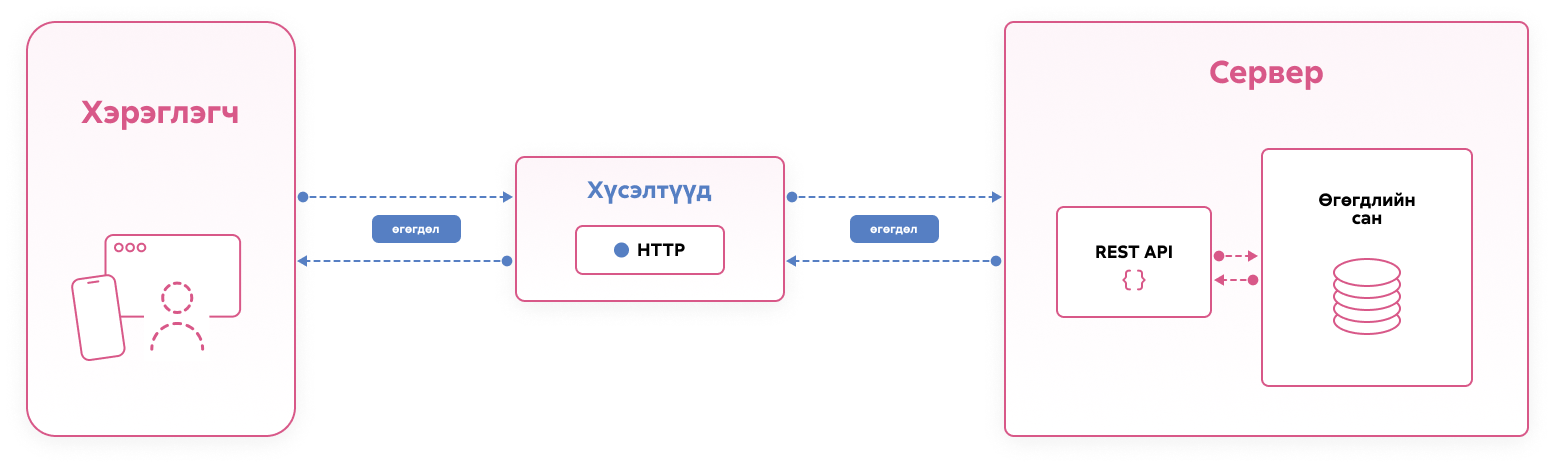
\includegraphics[width=15cm]{images/architecture.png}
	\caption{Three-tier Архитектурын үлгэр загварын дүрслэл}
	\label{fig:architecture}
\end{figure}

\clearpage

Front-end хэсэг Next.js дээр хөгжүүлэлт хийгдэх бол. Харин Back-end хэсэг Express.js болон Firebase дээр хөгжүүлэлт хийгдэнэ.

\begin{figure}[h]
	\centering
	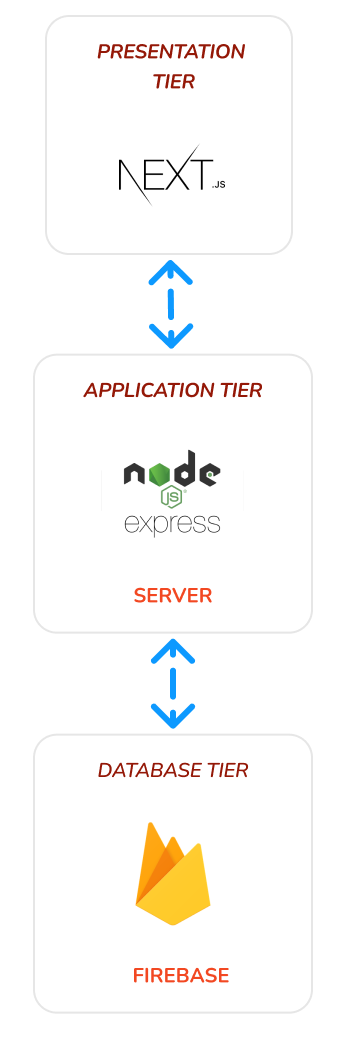
\includegraphics[scale=0.9]{images/imp-diag.png}
	\caption{Хэрэгжүүлэх гэж буй системийн архитектур}
	\label{fig:imp-architecture}
\end{figure}

% \begin{figure}[h]
% 	\centering
% 	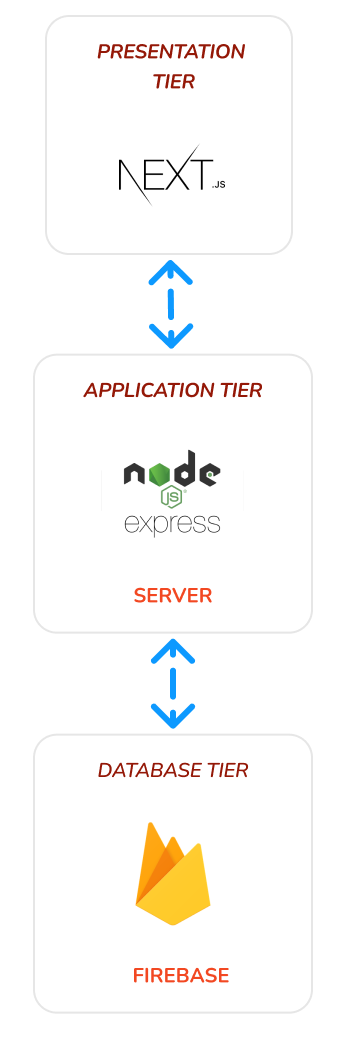
\includegraphics[width=0.8\textwidth]{images/imp-diag.png}
% 	\caption{Хэрэгжүүлэх гэж буй системийн архитектур}
% 	\label{fig:imp-architecture}
% \end{figure}



% \begin{itemize}
% 	\item Client талаас сервер рүү интернэт ашиглан HTTPS холболтоор өгөгдлөө дамжуулна
% 	\item Сервер дээр Prisma ORM-г ашиглан өгөгдлийн сангаа удирдана
% 	\item Хэрэглэгчээс орж ирсэн URL-г авч сервер нь гуравдагч сайтын мэдээллийг авахаар HTTPS холболтоор хүсэлт илгээн хариуд нь тухайн сайтын Open Graph Protocol дахь meta data-г авна.
% \end{itemize}


\pagebreak
\section{Ажлын явцын диаграм}

\subsection{Ажлын явцын диаграм}
% \begin{figure}[h]
% 	\centering
% 	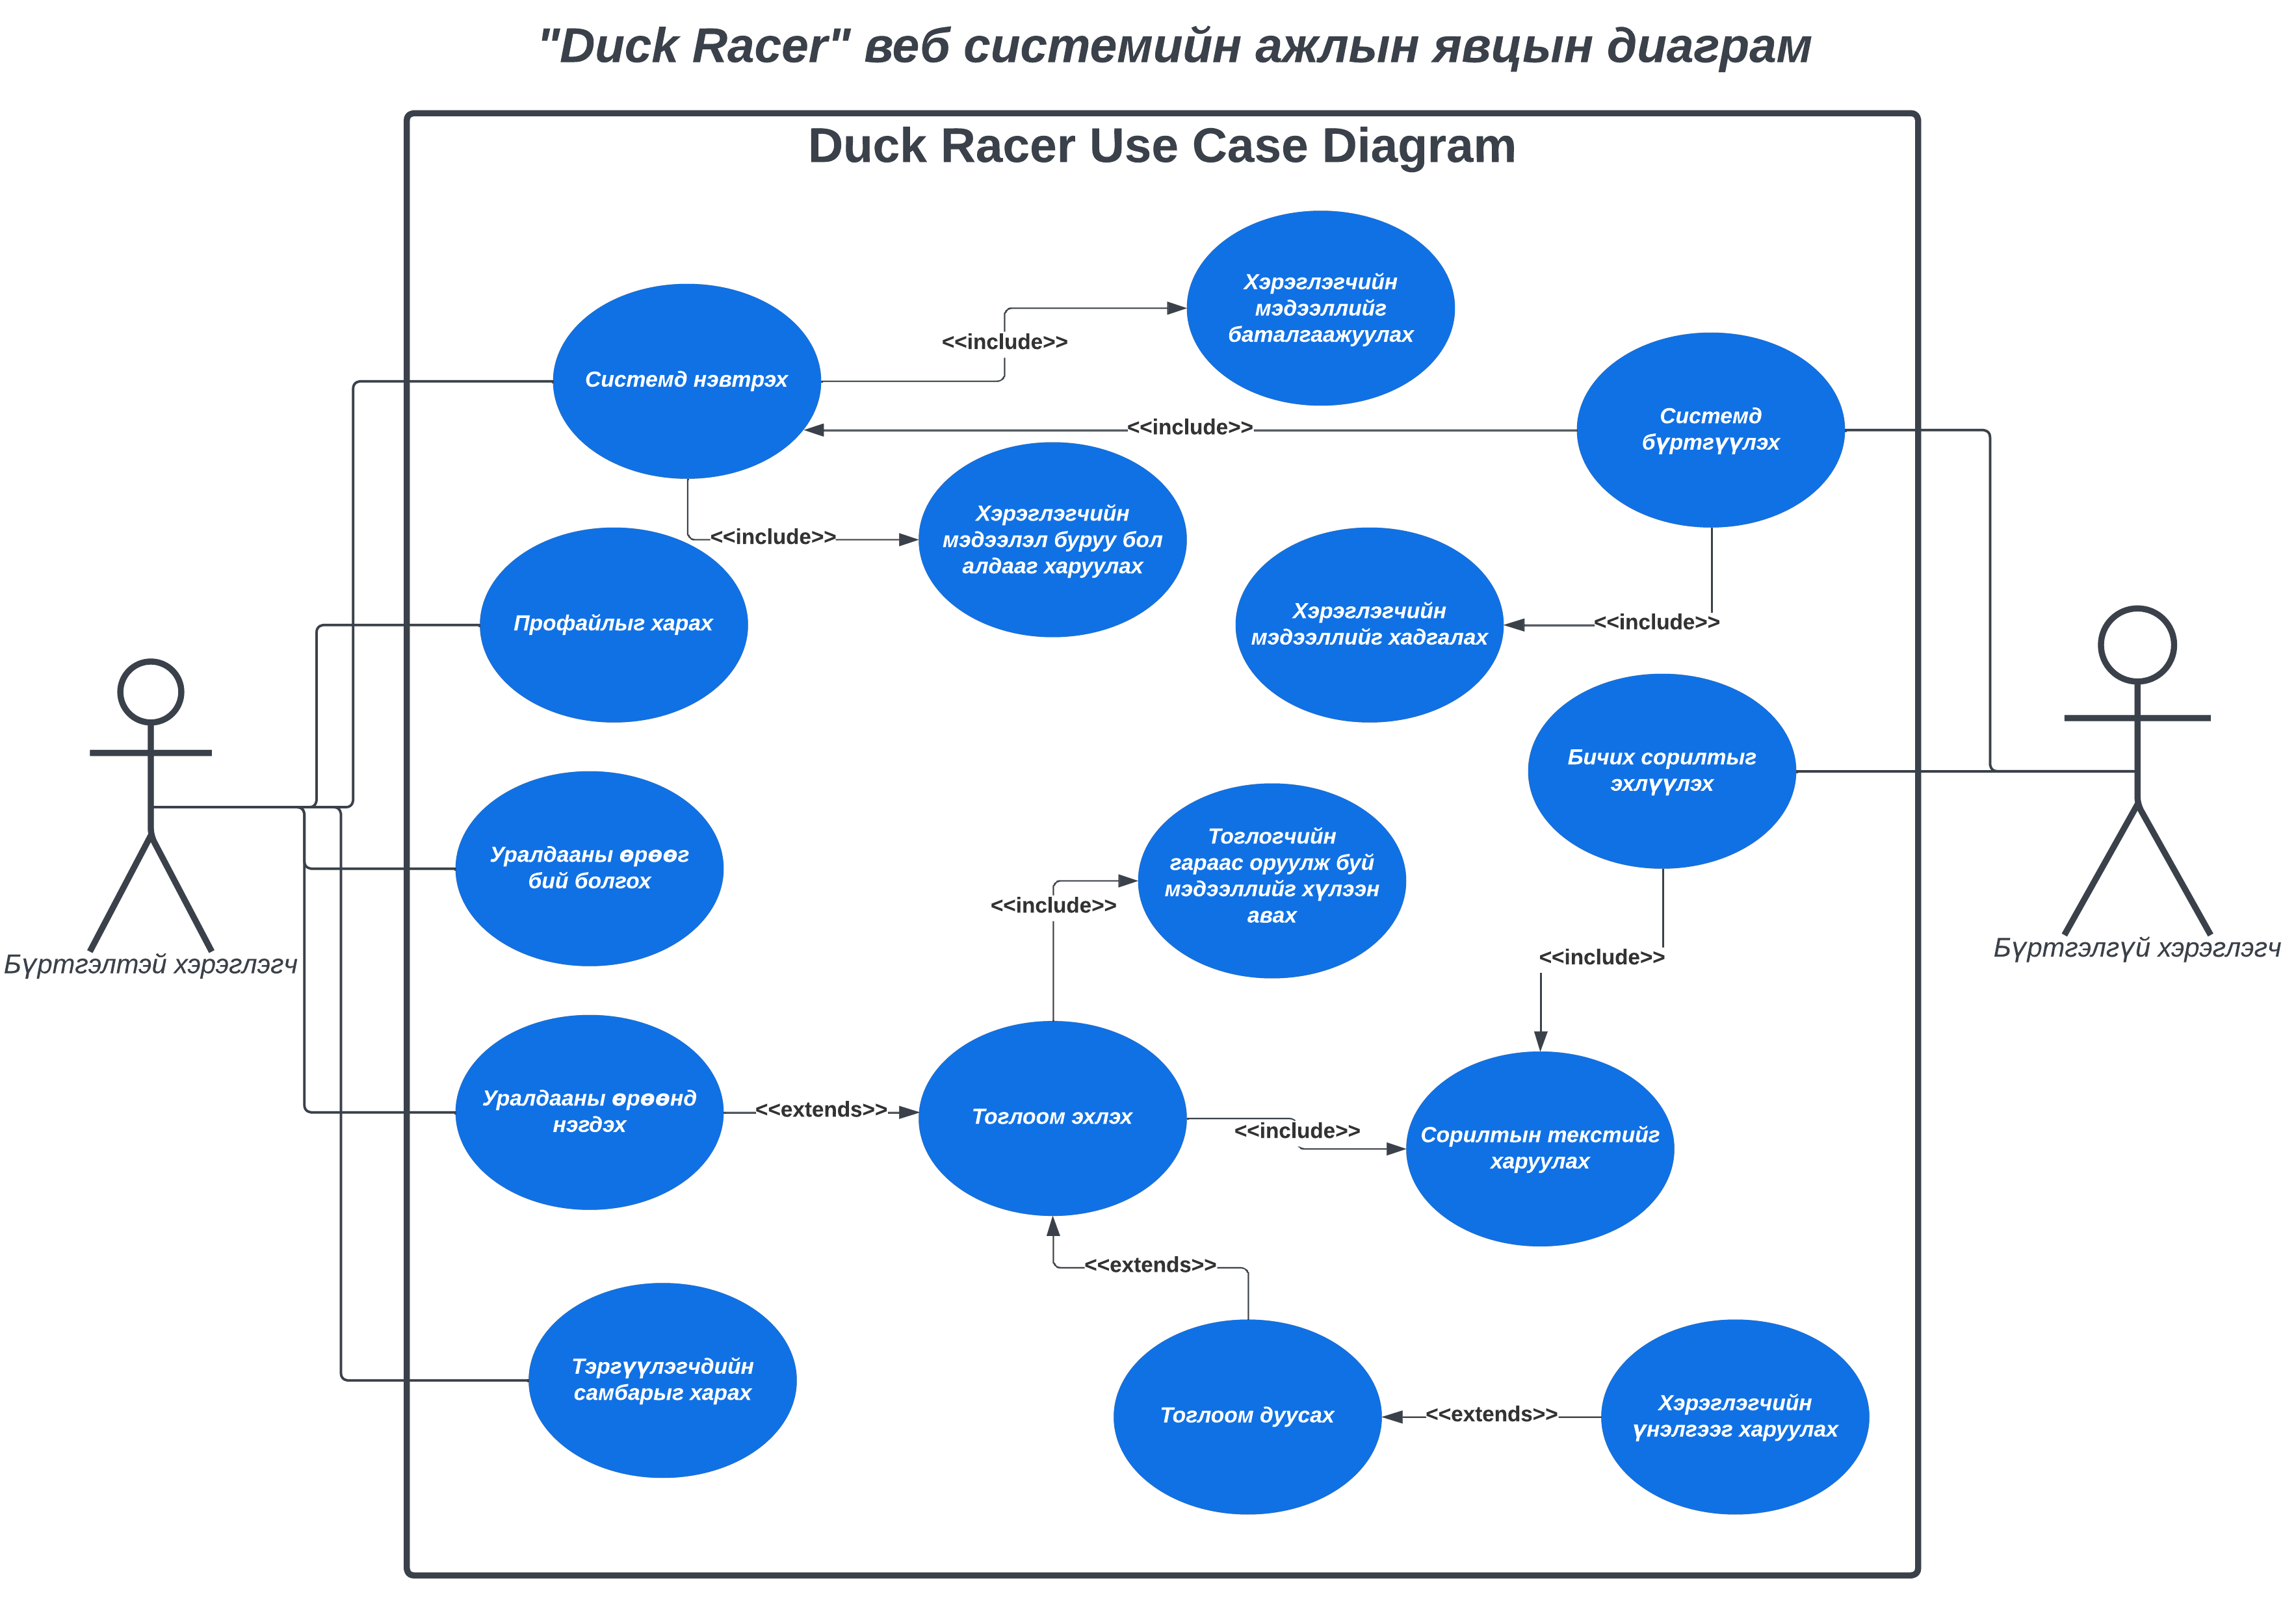
\includegraphics[width=15cm]{images/usecase.png}
% 	\caption{Ажлын явцын диаграм}
% 	\label{fig:usecase}
% \end{figure}

\textbf{Ажлын явцын диаграмын тайлбар}

\begin{itemize}
	\item \textbf{Нэвтрэх -} Бүртгүүлсэн хэрэглэгч системд хэрэглэгчийн нэр, нууц үгээ оруулан нэвтрэх
	\item \textbf{Профайлыг харах -} Бүртгэгдсэн хэрэглэгч өөрийн профайлыг харж бичих хурд, нарийвчлал болон бусад статистикийг харах
	\item \textbf{Бичих сорилтыг эхлүүлэх -} Бүх хэрэглэгч бичих чадвараа сайжруулахын тулд бичих сорилтыг эхлүүлэх
	\item \textbf{Тэргүүлэгчдийн самбарыг харах -} Бүртгүүлсэн хэрэглэгч тэргүүлэгчдийн самбарыг харж бусад хэрэглэгчдийнхээ эсрэг хэрхэн эрэмбэлэгдсэнийг харах
	\item \textbf{Уралдааны өрөөг бий болгох -} Бүртгүүлсэн хэрэглэгч бусад хэрэглэгчдийг шивэх уралдаанд уралдуулахын тулд уралдааны өрөө үүсгэх
	\item \textbf{Уралдааны өрөөнд нэгдэх -} Бүртгүүлсэн хэрэглэгч өөр хэрэглэгчийн үүсгэсэн уралдааны өрөөнд нэгдэх
	\item \textbf{Бүртгүүлэх -} Хэрэглэгч бүртгэлгүй хэдий ч манай платформыг бүрэн ашиглах боломжтой. Хэрэв өөрөө веб холбоос оруулахыг хүсвэл хувийн мэдээллээ бөглөж бүртгүүлэх
	\item \textbf{Сорилтын үр дүнг харах -} Бүртгэгдсэн хэрэглэгч шивэх сорилтынхоо үр дүнг харж, ахиц дэвшлийг нь харж, сайжруулах шаардлагатай хэсгийг тодорхойлох
\end{itemize}

\pagebreak
\section{UX/UI дизайн}

% Өмнөх бүлэгт хийсэн UX судалгаан дээрээ үндэслэж User Experience болон User Interface загварыг High Fidelity түвшинд эцэслэж гаргасан ба гаргасан дизайнаа хэрэглэгчээр туршиулж тодорхой үр дүнгүүдэд хүрч чадсан. Үүнд: 

% \begin{itemize}
% 	\item Хэрэглэгчийн шаардлагыг бүрэн ойлгож, хэрэглэгч төвтэй дизайн гаргасан
% 	\item Тусдаа бүлэг ажил болгон хийснээр интерфейс загвартаа анхаарч шинэлэг, ашиглахад хялбар хэрэглэгчийн интерфейс загвар зурсан
% 	\item Хөгжүүлэлтийн шатнаас өмнө бүх хэрэглэгчийн интерфейсүүд дизайн системийн дагуу гарч дууссан тул front-end хөгжүүлэлтийн явцыг ихээр хурдлуулсан
% 	\item Интерфейсийн дагуу front-end код явагдах тул back-end код дээр dummy датагаар хөгжүүлж явах, төлөвлөх үе шат хялбар болсон. Front-end хэсэгтэй зөрөх магадлал багассан гэж ойлгож болно.
% \end{itemize}

% Одоо UX шаардлагын дагуу ажилласан процессоо богиноор тайлбарлая.

% \subsection{User Persona тодорхойлж эхний загварыг бүтээсэн нь}

% Шаардлагын дагуу хоёр хүнийг сонгон авч тэдгээр хүмүүсээс хэрэгтэй мэдээллүүдээ нэгтгэсэн ба доорхи зургаар илэрхийллээ.

% \textbf{User Persona 1 - Болорчулуун}

% \begin{figure}[h]
% 	\centering
% 	
\includegraphics[width=15cm]{images/persona1-bolorchuluun.png}
% 	\caption{Persona 1 - Болорчулууны мэдээлэл}
% 	\label{fig:persona1}
% \end{figure}

% \textbf{Use Case}

% \begin{itemize}
% 	\item Өглөө ажил дээрээ эхний 20 минут мэргэжилтэйгээ холбоотой нийтлэлүүд унших дуртай
% 	\item Веб хөтөч дээрээ таалагдсан эсвэл дараа нь унших ёстой холбоосуудаа bookmark хийж хадгалж авдаг боловч зөвхөн ажлын компьютер дээр л тэдгээр холбоос маань хадгалагддаг. Өөр рүүгээ веб холбоосоо цуглуулж явуулахаас залхуу хүрдэг
% \end{itemize}

% \textbf{User Persona 2 - Шүрэнцэцэгийн мэдээлэл}

% \begin{figure}[h]
% 	\centering
% 	
\includegraphics[width=15cm]{images/persona2-shurentsetseg.png}
% 	\caption{Persona 2 - Шүрэнцэцэг}
% 	\label{fig:persona2}
% \end{figure}

% \textbf{Use Case}

% \begin{itemize}
% 	\item Миний хувьд мэдээгээ бэлтгэхдээ дийлэнхдээ интернет дэх эх сурвалжуудаас бэлтгэдэг. Нэг асуудал байдаг маань эх сурвалж авдаг хэдхэн вэбсайт дунд л эргэлдэж байгаа.
% 	\item Олсон мэдээллүүдээ хамт ажиллаж буй хүмүүс рүүгээ явуулахдаа Telegram ашиглан нэг нэгээр нь хуулж тавин явуулдаг. Хүн болгон руу ингэж явуулах нь надад төвөгтэй байдаг
% \end{itemize}

% \textbf{Эхний Wireframe загварыг гаргаж Prototype хувилбар бүтээсэн нь}

% Хамгийн эхэнд нийт 8 хуудсын Wireframe загварыг хэрэглэгчийн Use Case дээрээ тулгуурлан зурж, дизайн дээрх бүх элементүүдээ хооронд нь холбон Prototype \footnote{Prototype хувилбарыг туршиж үзэх \url{https://www.figma.com/proto/EL2nOGmToBRVxHNuZwH661/Draft?}} хувилбар гаргаж, сонгож авсан хоёр хэрэглэгч дээрээ Usability туршилт хийхэд бэлэн болголоо.

% Нийт зурсан 8 хуудсаас вебийн гол процессийг илэрхийлэх 4 зургийг орууллаа. Бусад хэсгийг хавсралтаас \footnote{Зурсан интерфейс дизайн \url{https://www.figma.com/file/EL2nOGmToBRVxHNuZwH661}} үзэх боломжтой

% \begin{figure}[h]
% 	\centering
% 	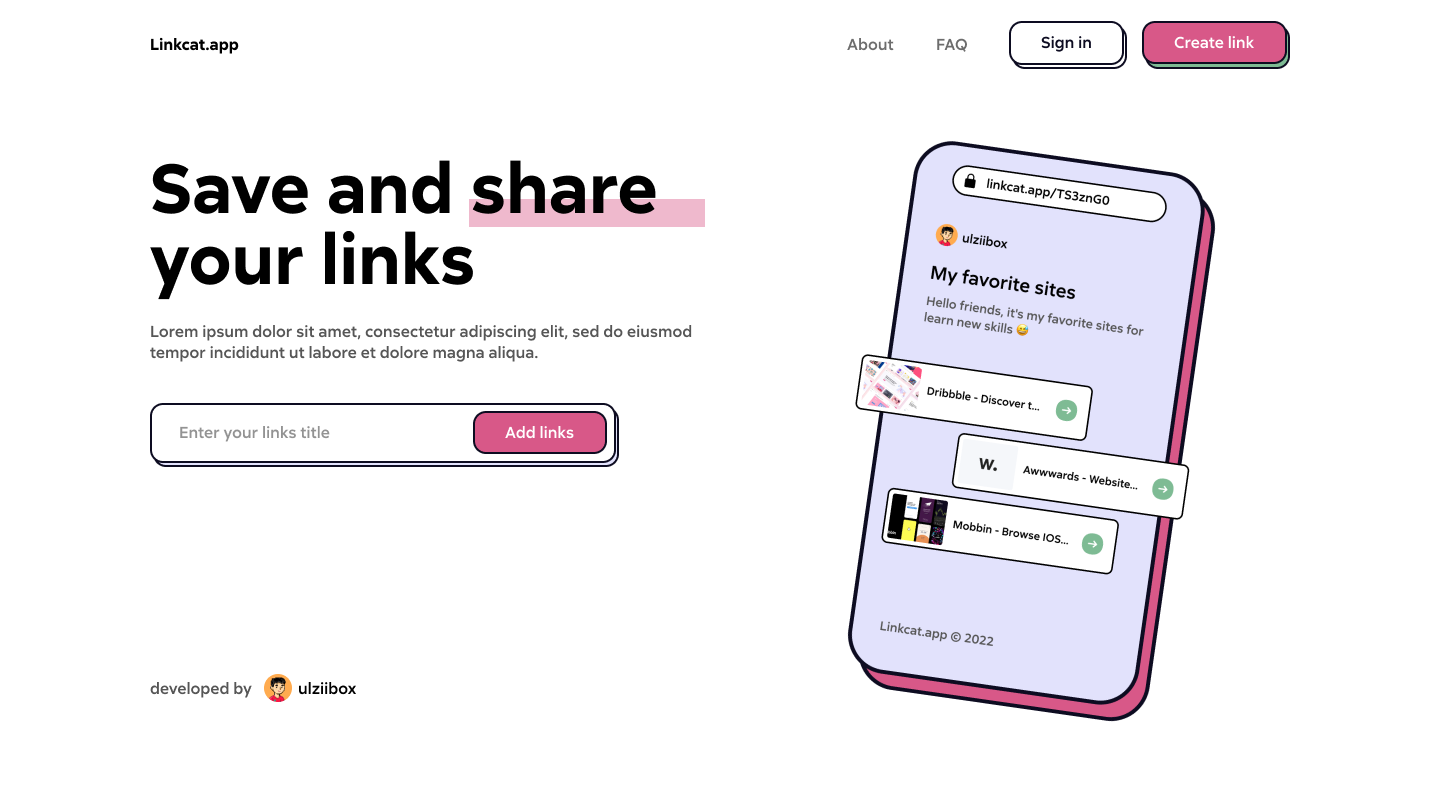
\includegraphics[width=10cm]{images/interfaces/v1/01-home.png}
% 	\caption{Нүүр хуудас}
% 	\label{fig:interface-v1-01}
% \end{figure}

% \begin{figure}[h]
% 	\centering
% 	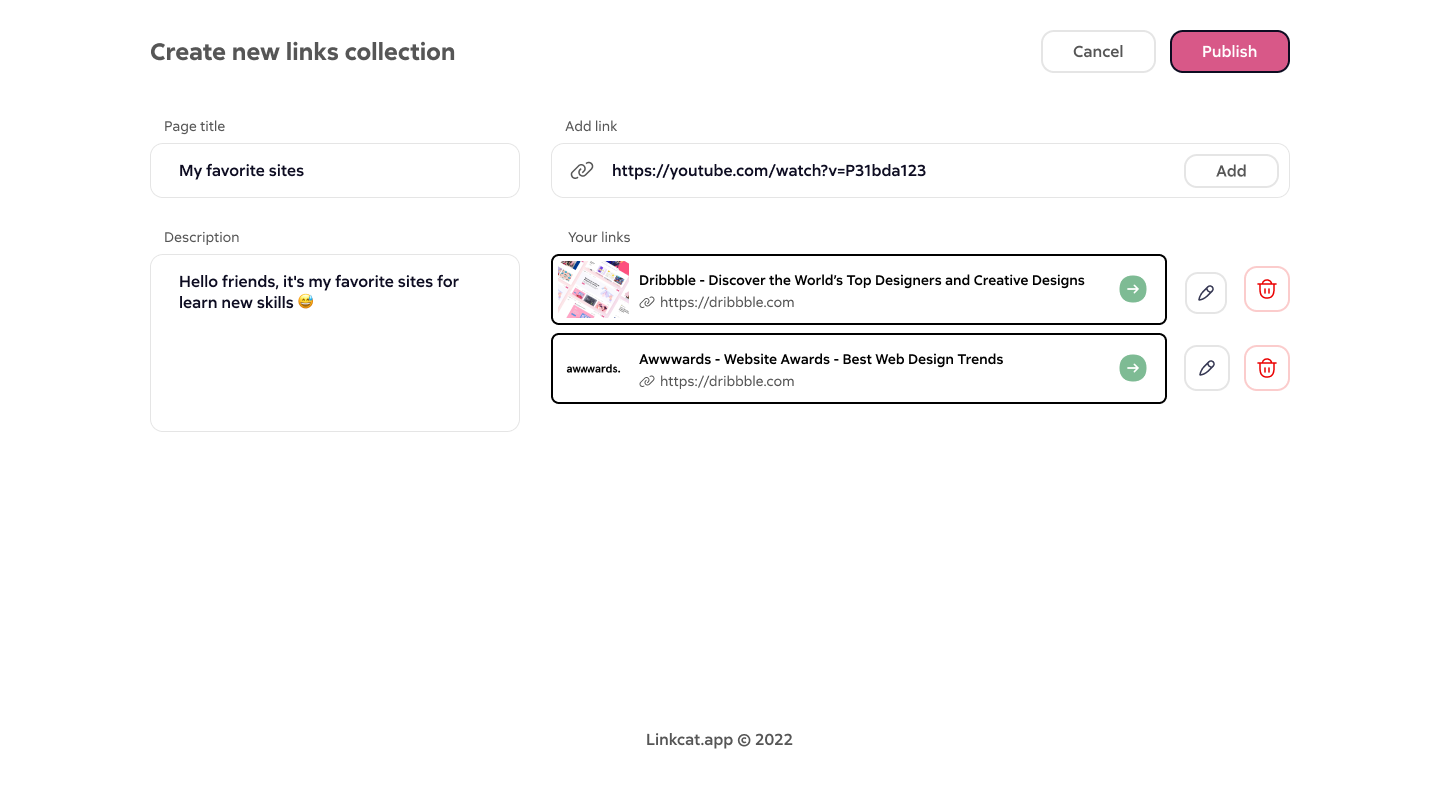
\includegraphics[width=10cm]{images/interfaces/v1/02-interface-createlink.png}
% 	\caption{Холбоосуудаа оруулах форм}
% 	\label{fig:interface-v1-02}
% \end{figure}

% \begin{figure}[h]
% 	\centering
% 	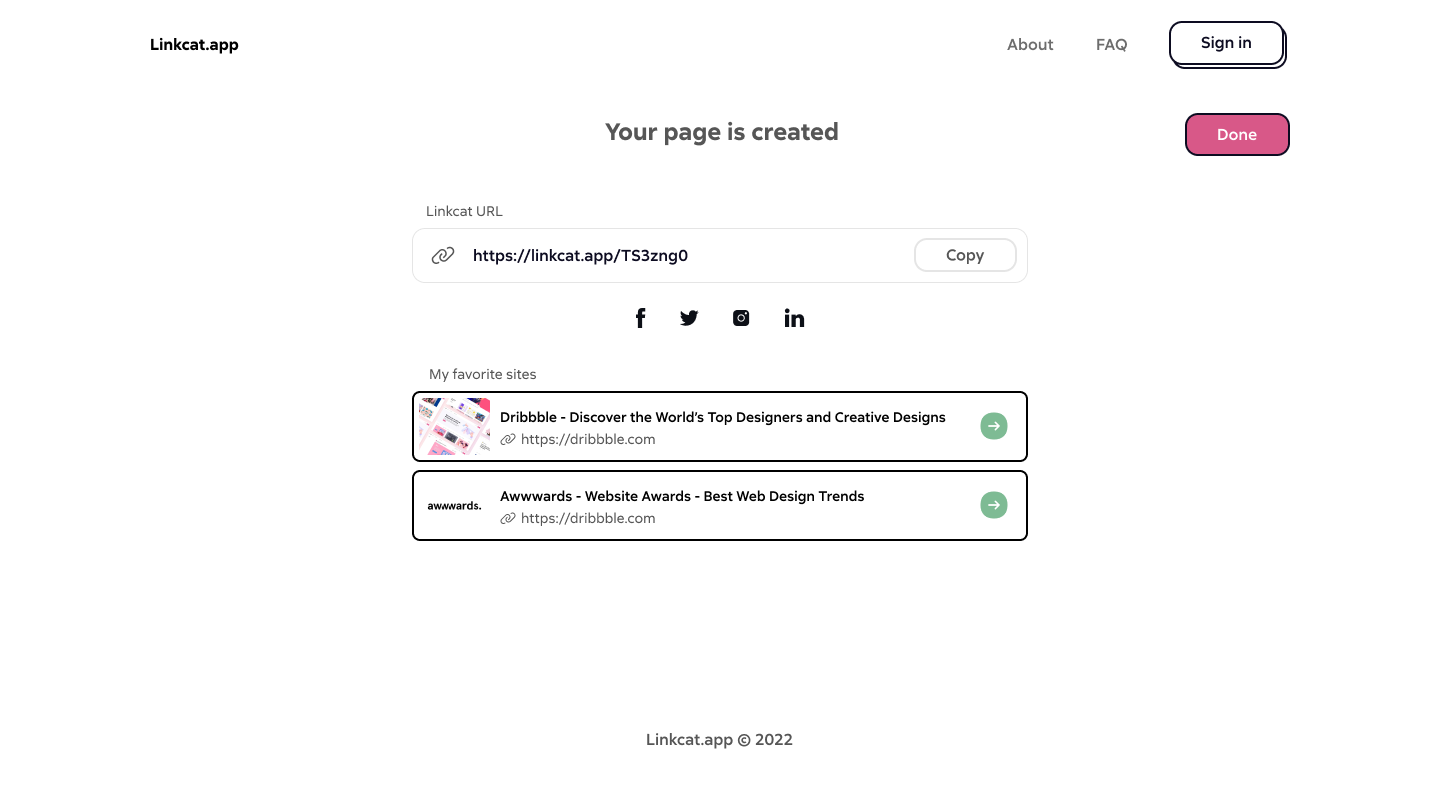
\includegraphics[width=10cm]{images/interfaces/v1/03-publis.png}
% 	\caption{Оруулсан холбоосуудыг нийтлэсний дараах хуудас}
% 	\label{fig:interface-v1-03}
% \end{figure}

% \begin{figure}[h]
% 	\centering
% 	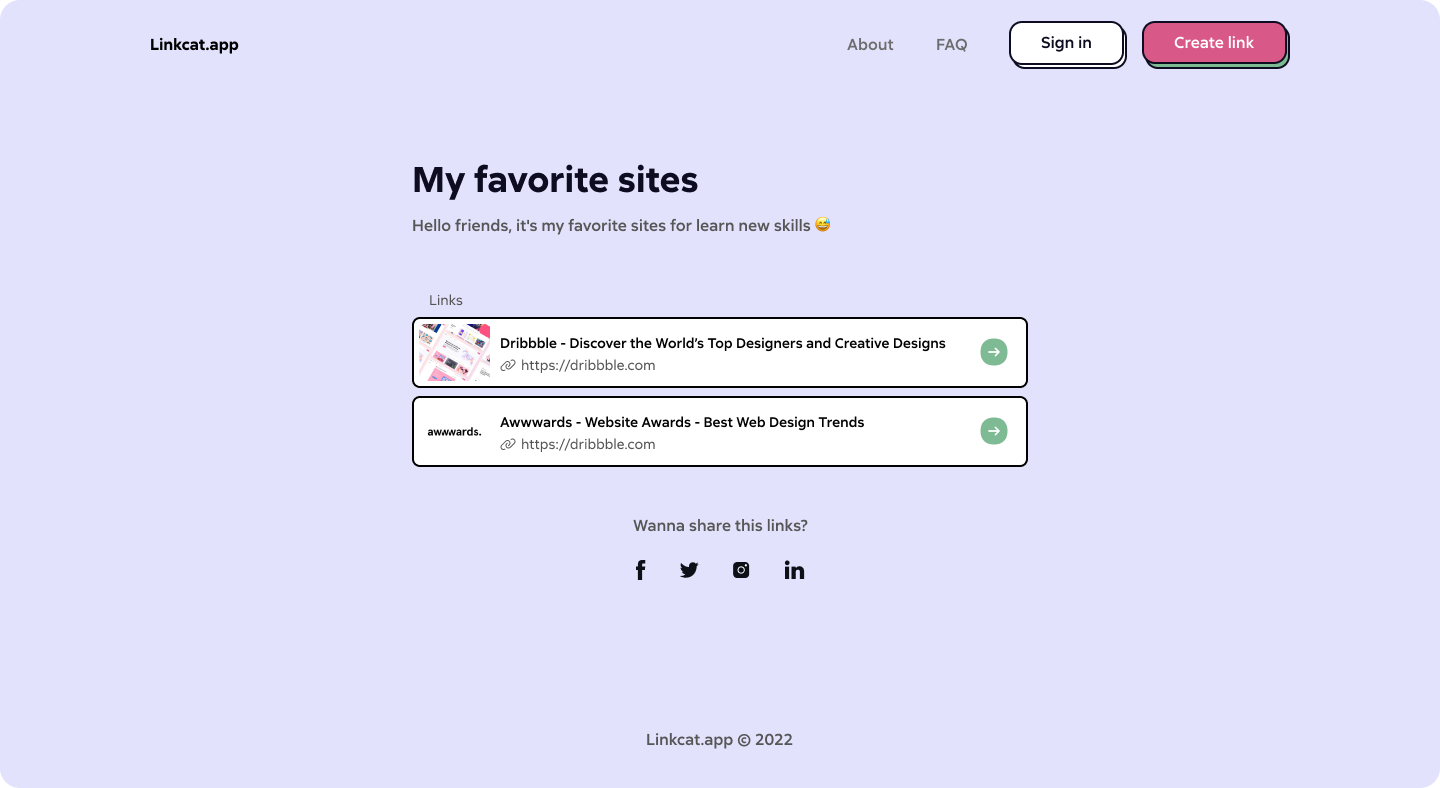
\includegraphics[width=10cm]{images/interfaces/v1/04-link-list.png}
% 	\caption{Оруулсан нийтлэл бусад хүмүүст харагдах байдал}
% 	\label{fig:interface-v1-04}
% \end{figure}

% \clearpage
% \textbf{Prototype хувилбар дээрээ Usability туршилт хийсэн нь}

% Дараа нь Prototype хувилбар дээрээ Usability буюу хэрэглэхэд тухтай байдлын туршилтыг сонгож авсан хоёр хэрэглэгч дээрээ хийлгэж уг гаргасан дизайн дээрх үүссэн асуудлыг тодорхойлж, хэрэглэгчээс санал хүсэлтийг аван дараагийн гаргах дизайныхаа ерөнхий шаардлагуудыг тодорхойлов. Үүнээс дурдвал:

% \begin{itemize}
% 	\item UI загварын хувьд концептийг дахин сайжруулах
% 	\item Бусад хүмүүсийн оруулсан холбоосыг нийтэд нь харуулах
% 	\item Оруулж буй холбоосыг ангилалтай байлгах
% 	\item Платформ дээр бүртгэлтэй бусад хэрэглэгчдийг харуулах
% \end{itemize}

% Иймд уг шаардлага дээрээ үндэслэн эцсийн байдлаар вебийнхээ UX/UI дизайныг гаргах шаардлагатай.

% \textbf{Redesign буюу зурсан дизайнаа дахин сайжруулсан нь}

% UX/UI гүйцэтгэлийн хамгийн сүүлийн шатанд нийт 12 хуудас дизайныг \footnote{UX/UI дизайны сүүлийн хувилбар \url{https://www.figma.com/proto/EL2nOGmToBRVxHNuZwH661}} холбож зурсан ба өмнөх дизайны процесстой адилаар Prototype хувилбар гаргаж эцсийн хэрэглэгчдээрээ Usability туршилтыг хийж дараагийн шат болох код хөгжүүлэлтийн шатыг эхлүүлэхэд бэлэн боллоо. Нийт зурсан хуудсаасаа 6 хуудсыг онцлон харуулж, User Expierence дизайныхаа шийдлийг тайлбарлалаа. Бусад зурсан хуудсыг доор байгаа хавсралтаас харах боломжтой. 

% \begin{figure}[h]
% 	\centering
% 	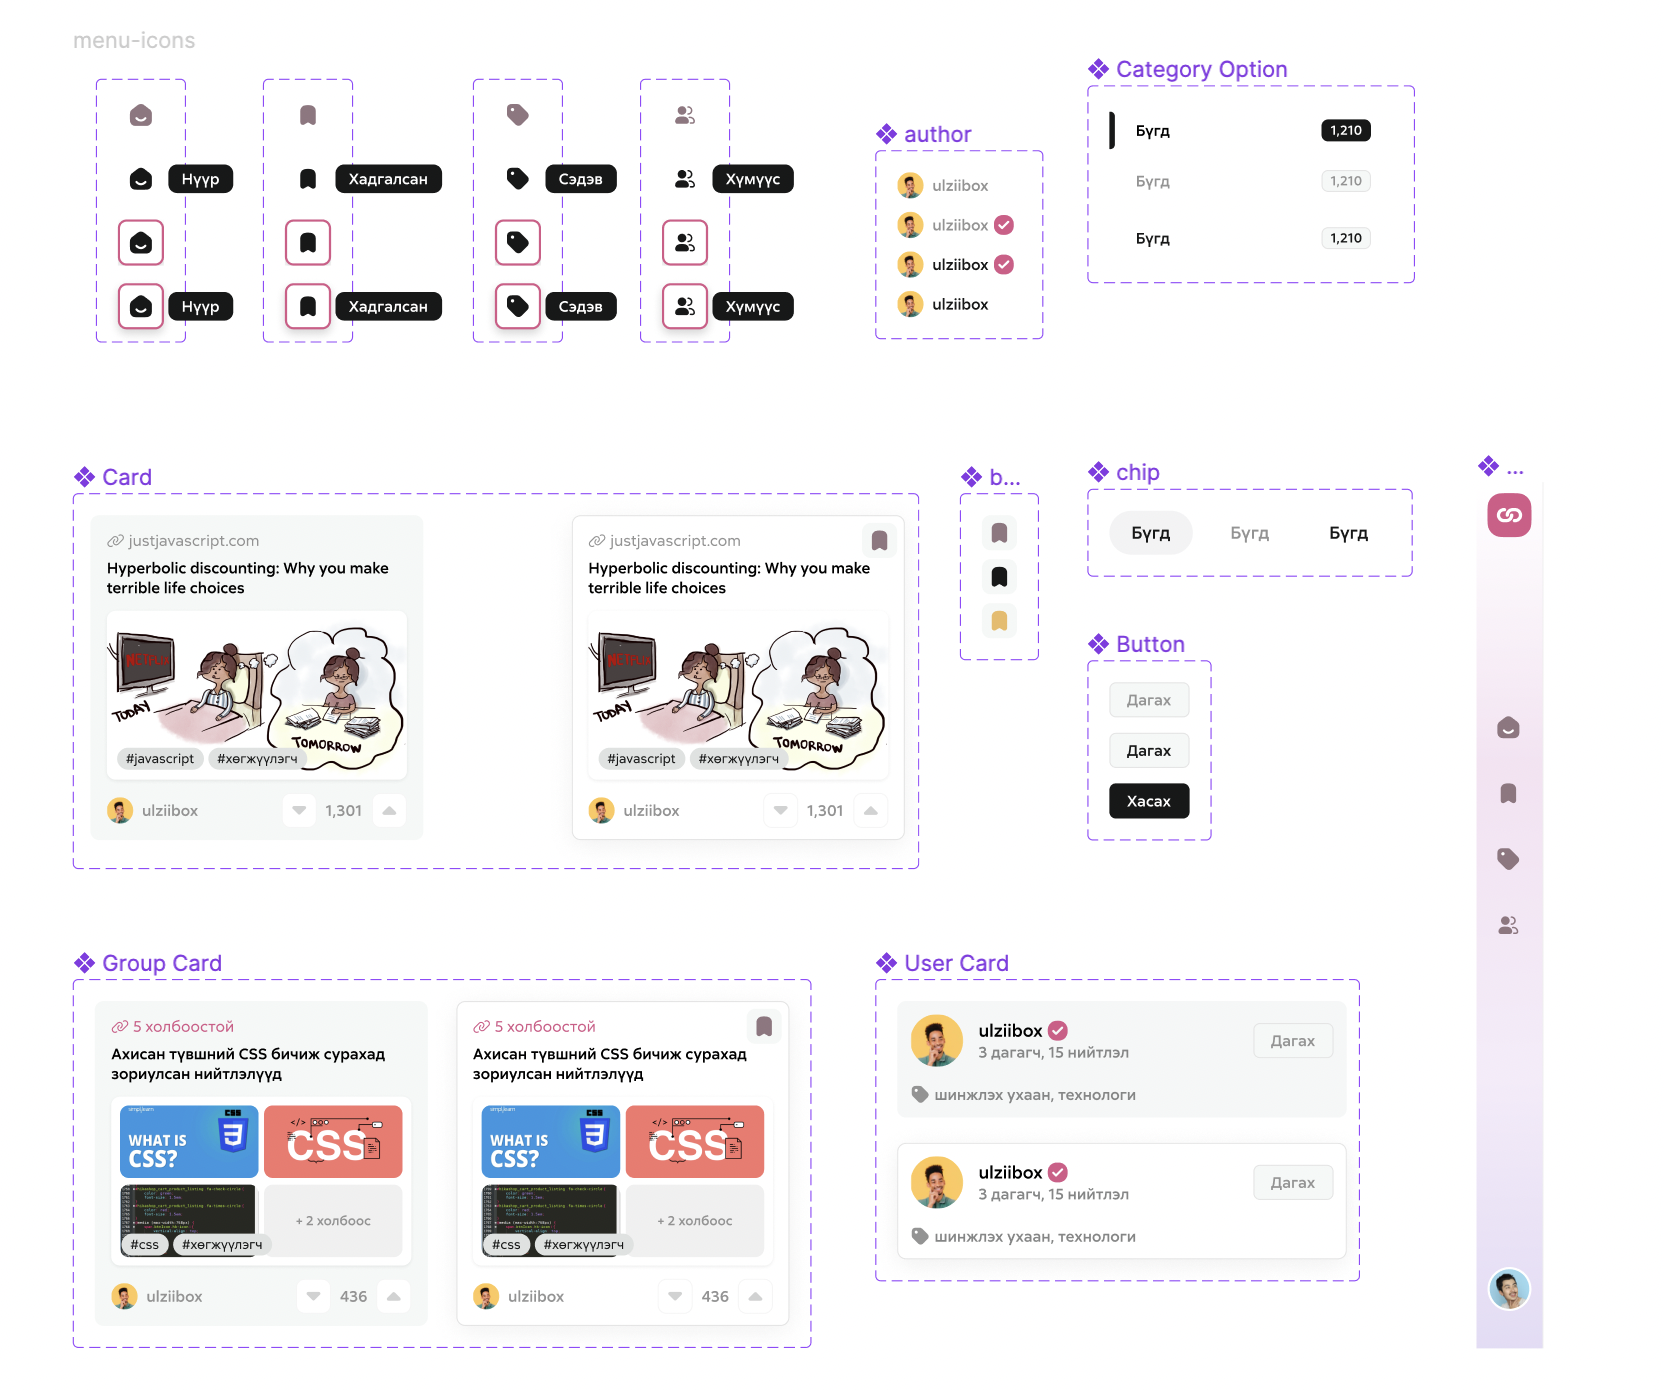
\includegraphics[width=10cm]{images/interfaces/components.png}
% 	\caption{Ашигласан компонентуудын жишээ}
% 	\label{fig:component}
% \end{figure}

% \begin{figure}[h]
% 	\centering
% 	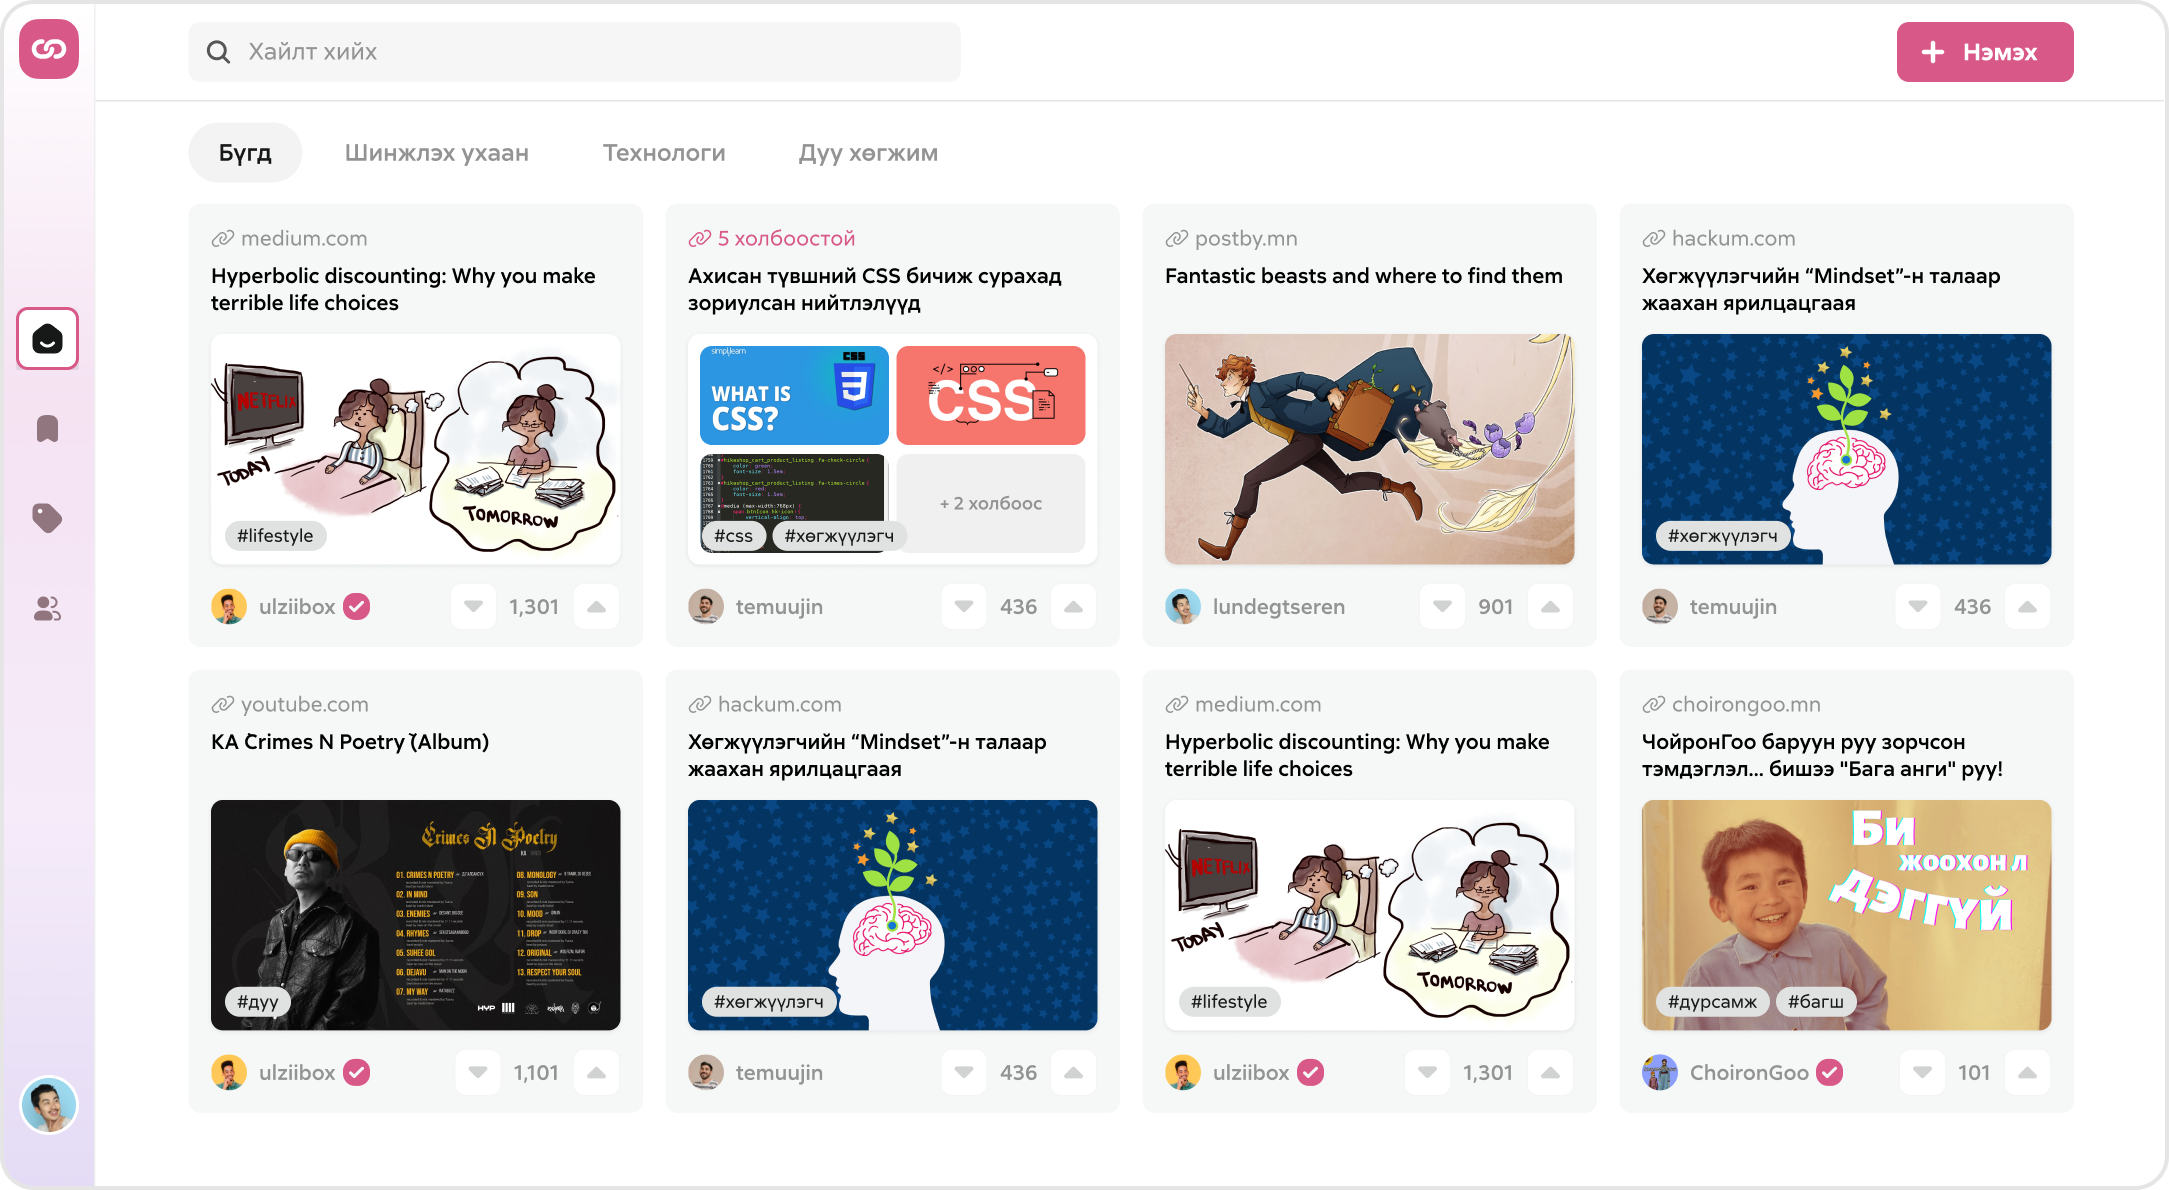
\includegraphics[width=10cm]{images/interfaces/home-screen.png}
% 	\caption{Нэвтэрсний дараах нүүр хуудас}
% 	\label{fig:homescreen}
% \end{figure}

% \begin{figure}[h]
% 	\centering
% 	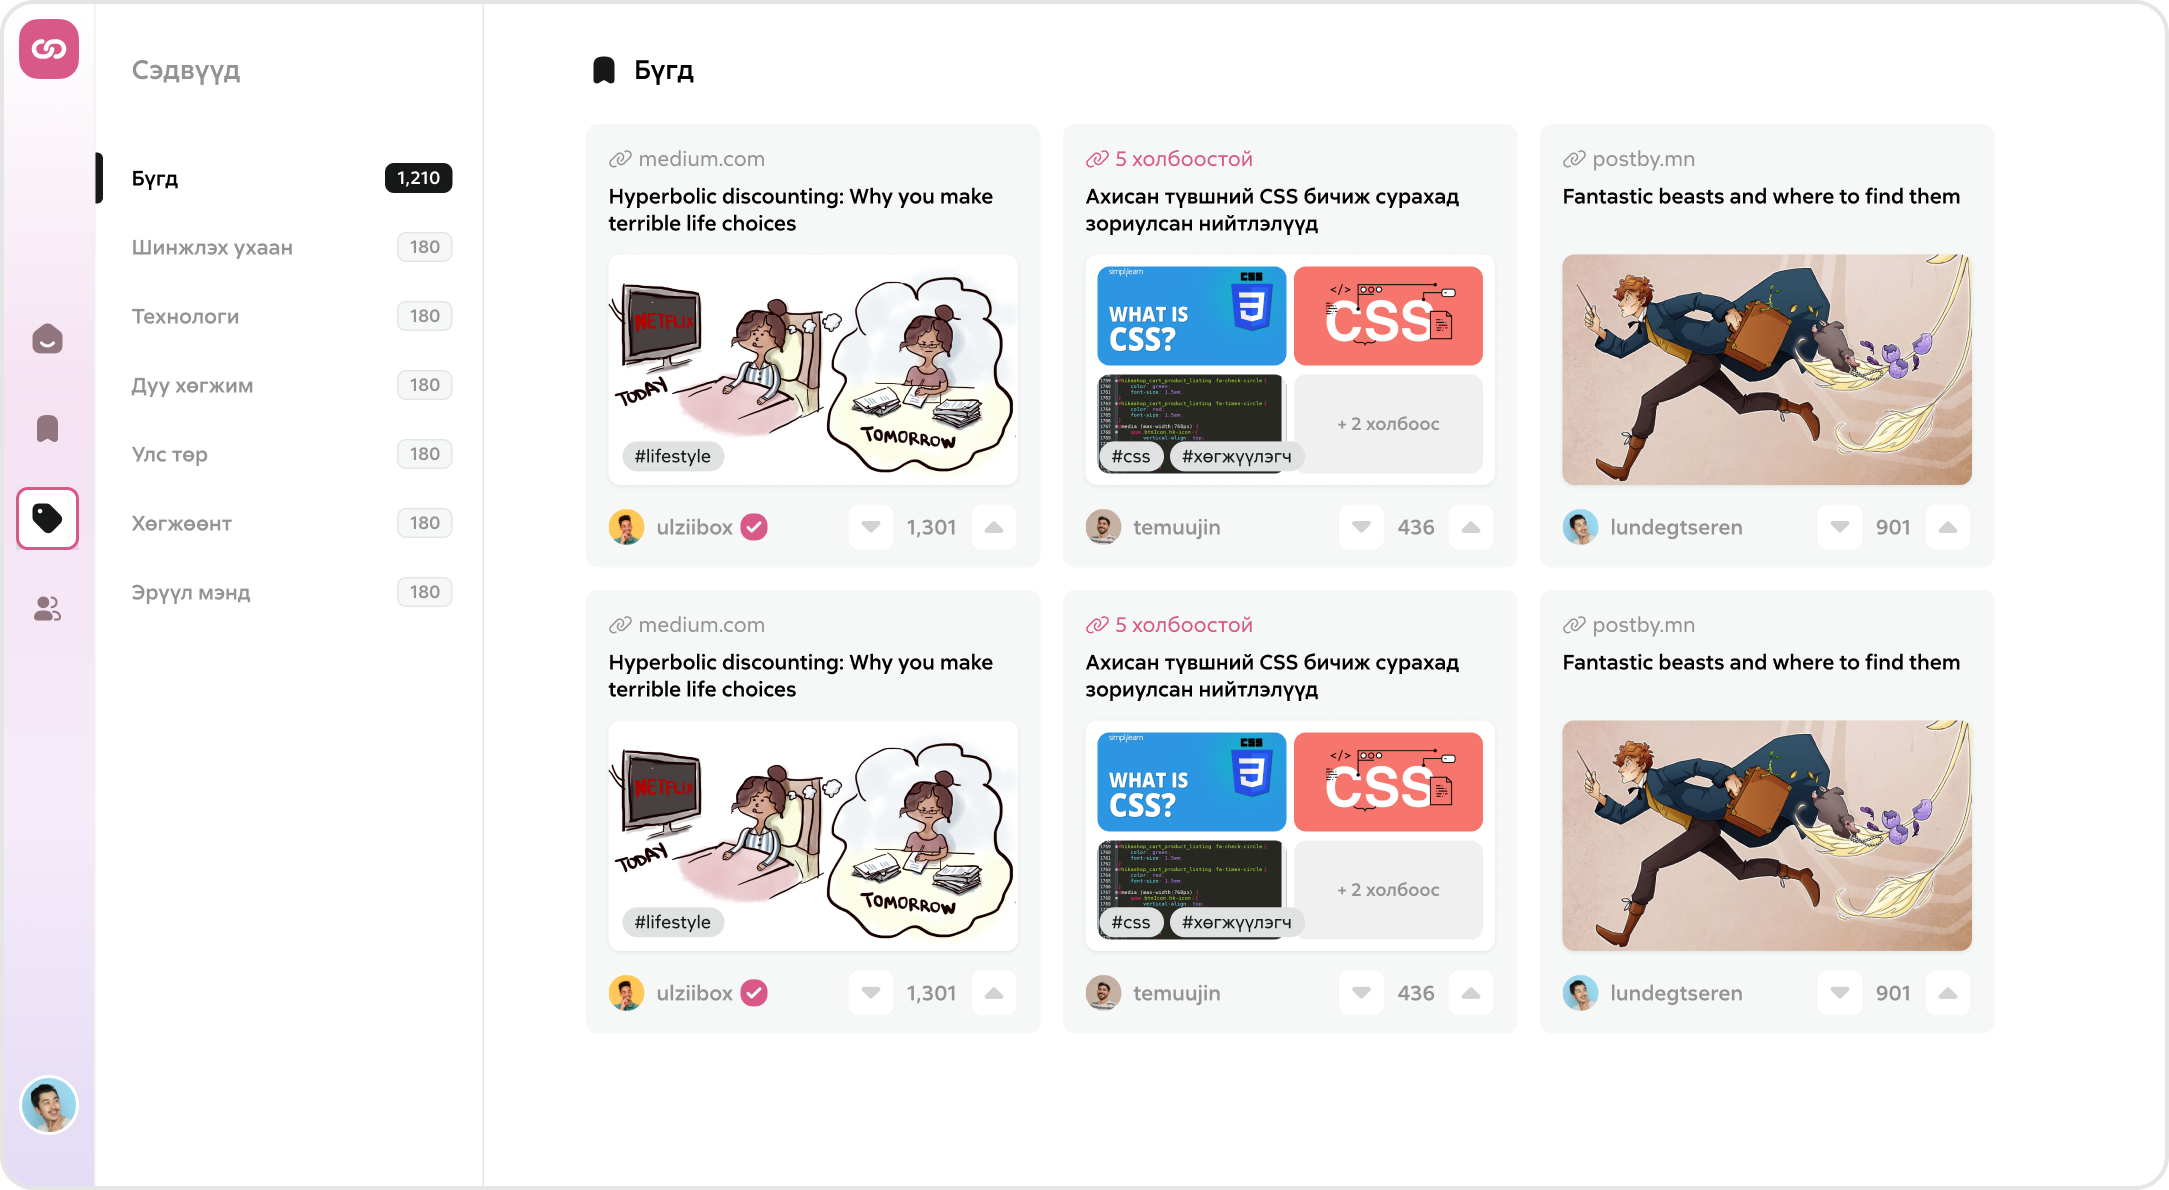
\includegraphics[width=10cm]{images/interfaces/topics.png}
% 	\caption{Бүх холбоосуудыг төрлөөр нь шүүж харах хуудас}
% 	\label{fig:topics}
% \end{figure}

% \begin{figure}[h]
% 	\centering
% 	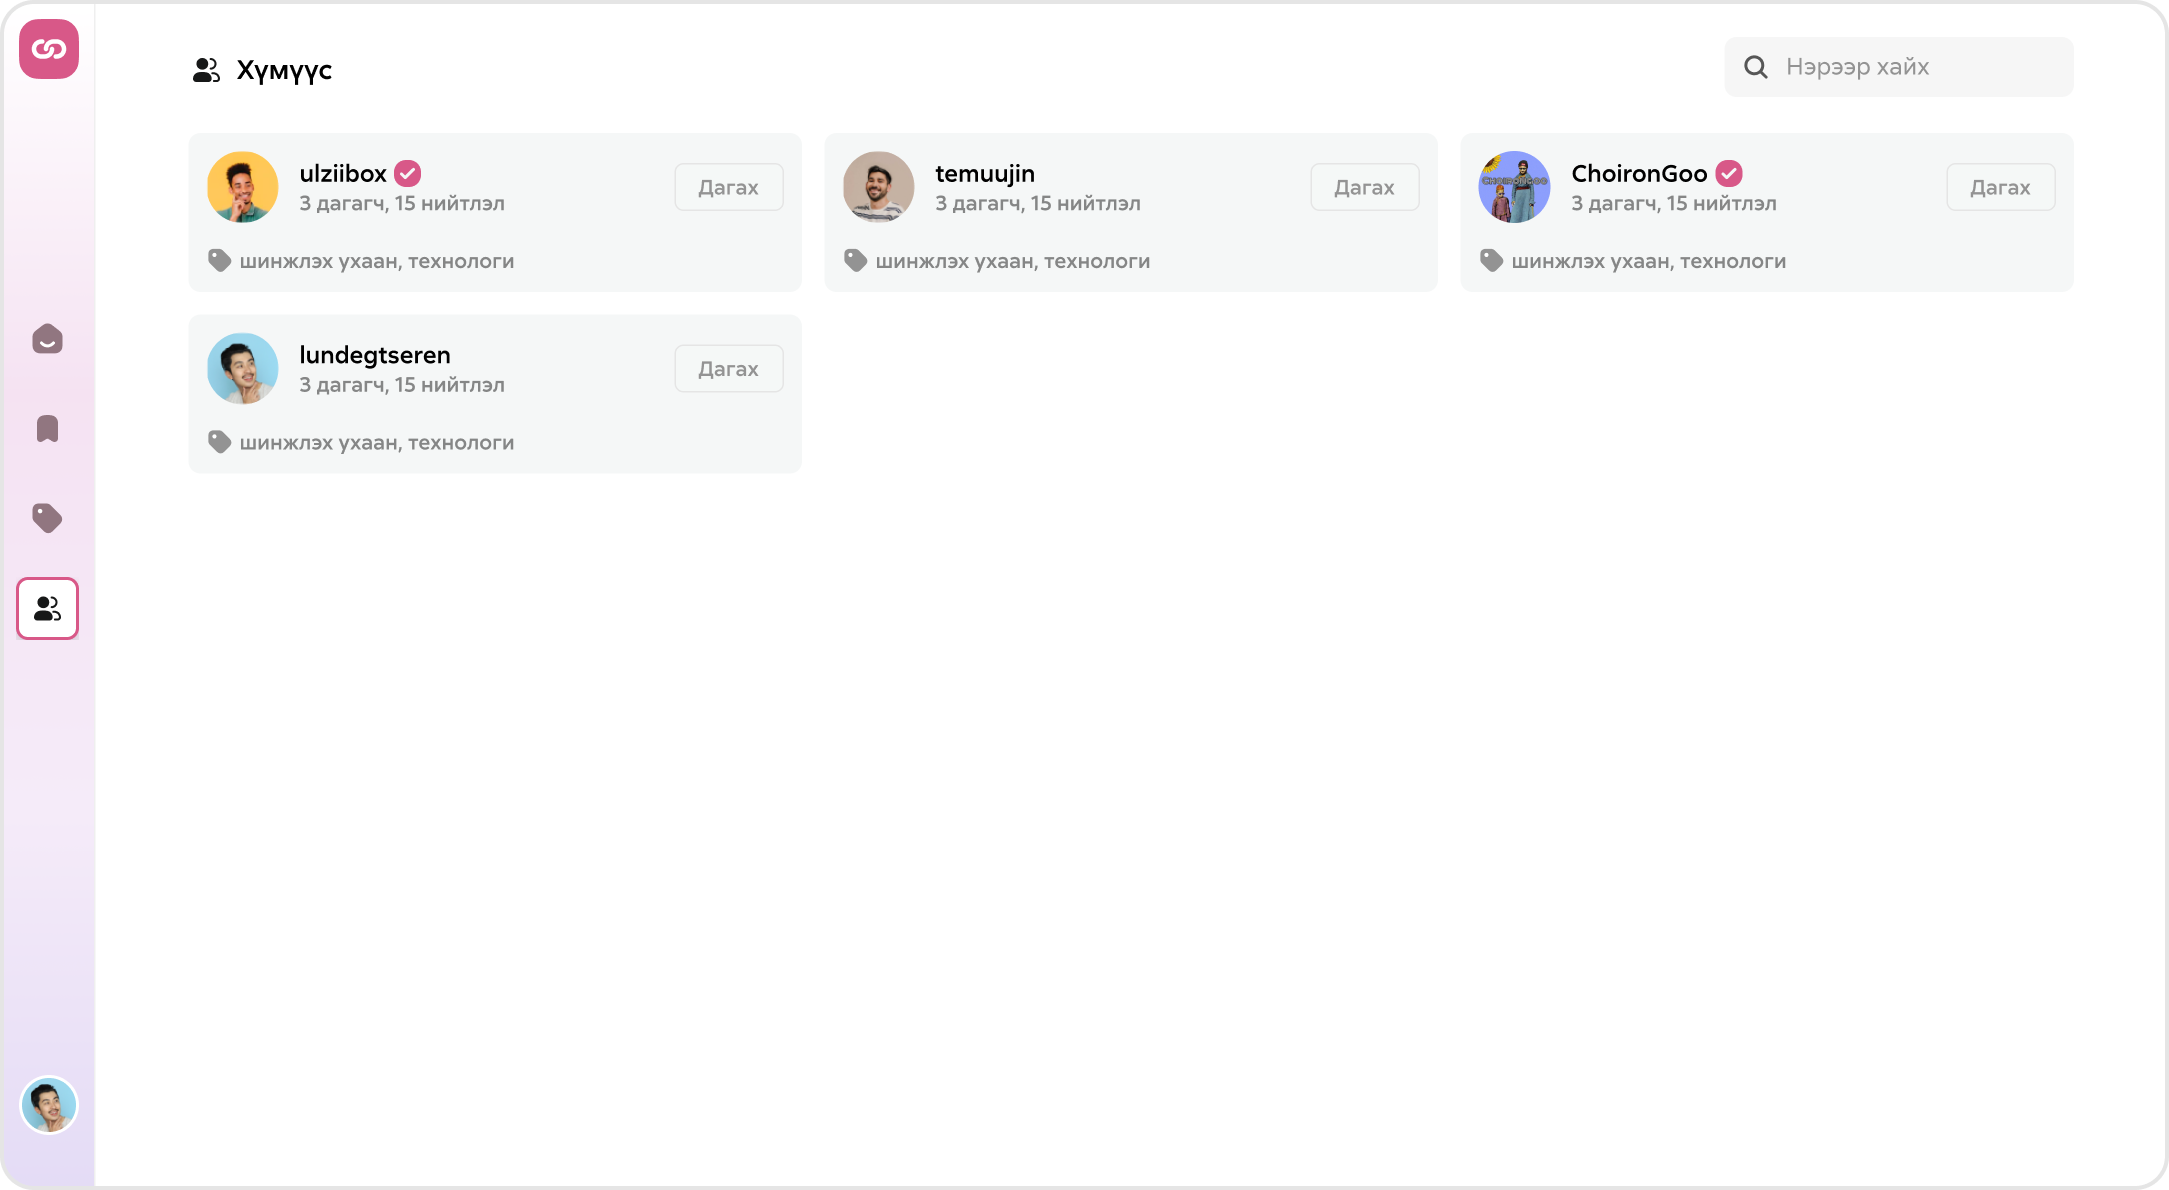
\includegraphics[width=10cm]{images/interfaces/people.png}
% 	\caption{Хэрэглэгчдийн жагсаалт харагдах хуудас}
% 	\label{fig:people}
% \end{figure}

% \begin{figure}[h]
% 	\centering
% 	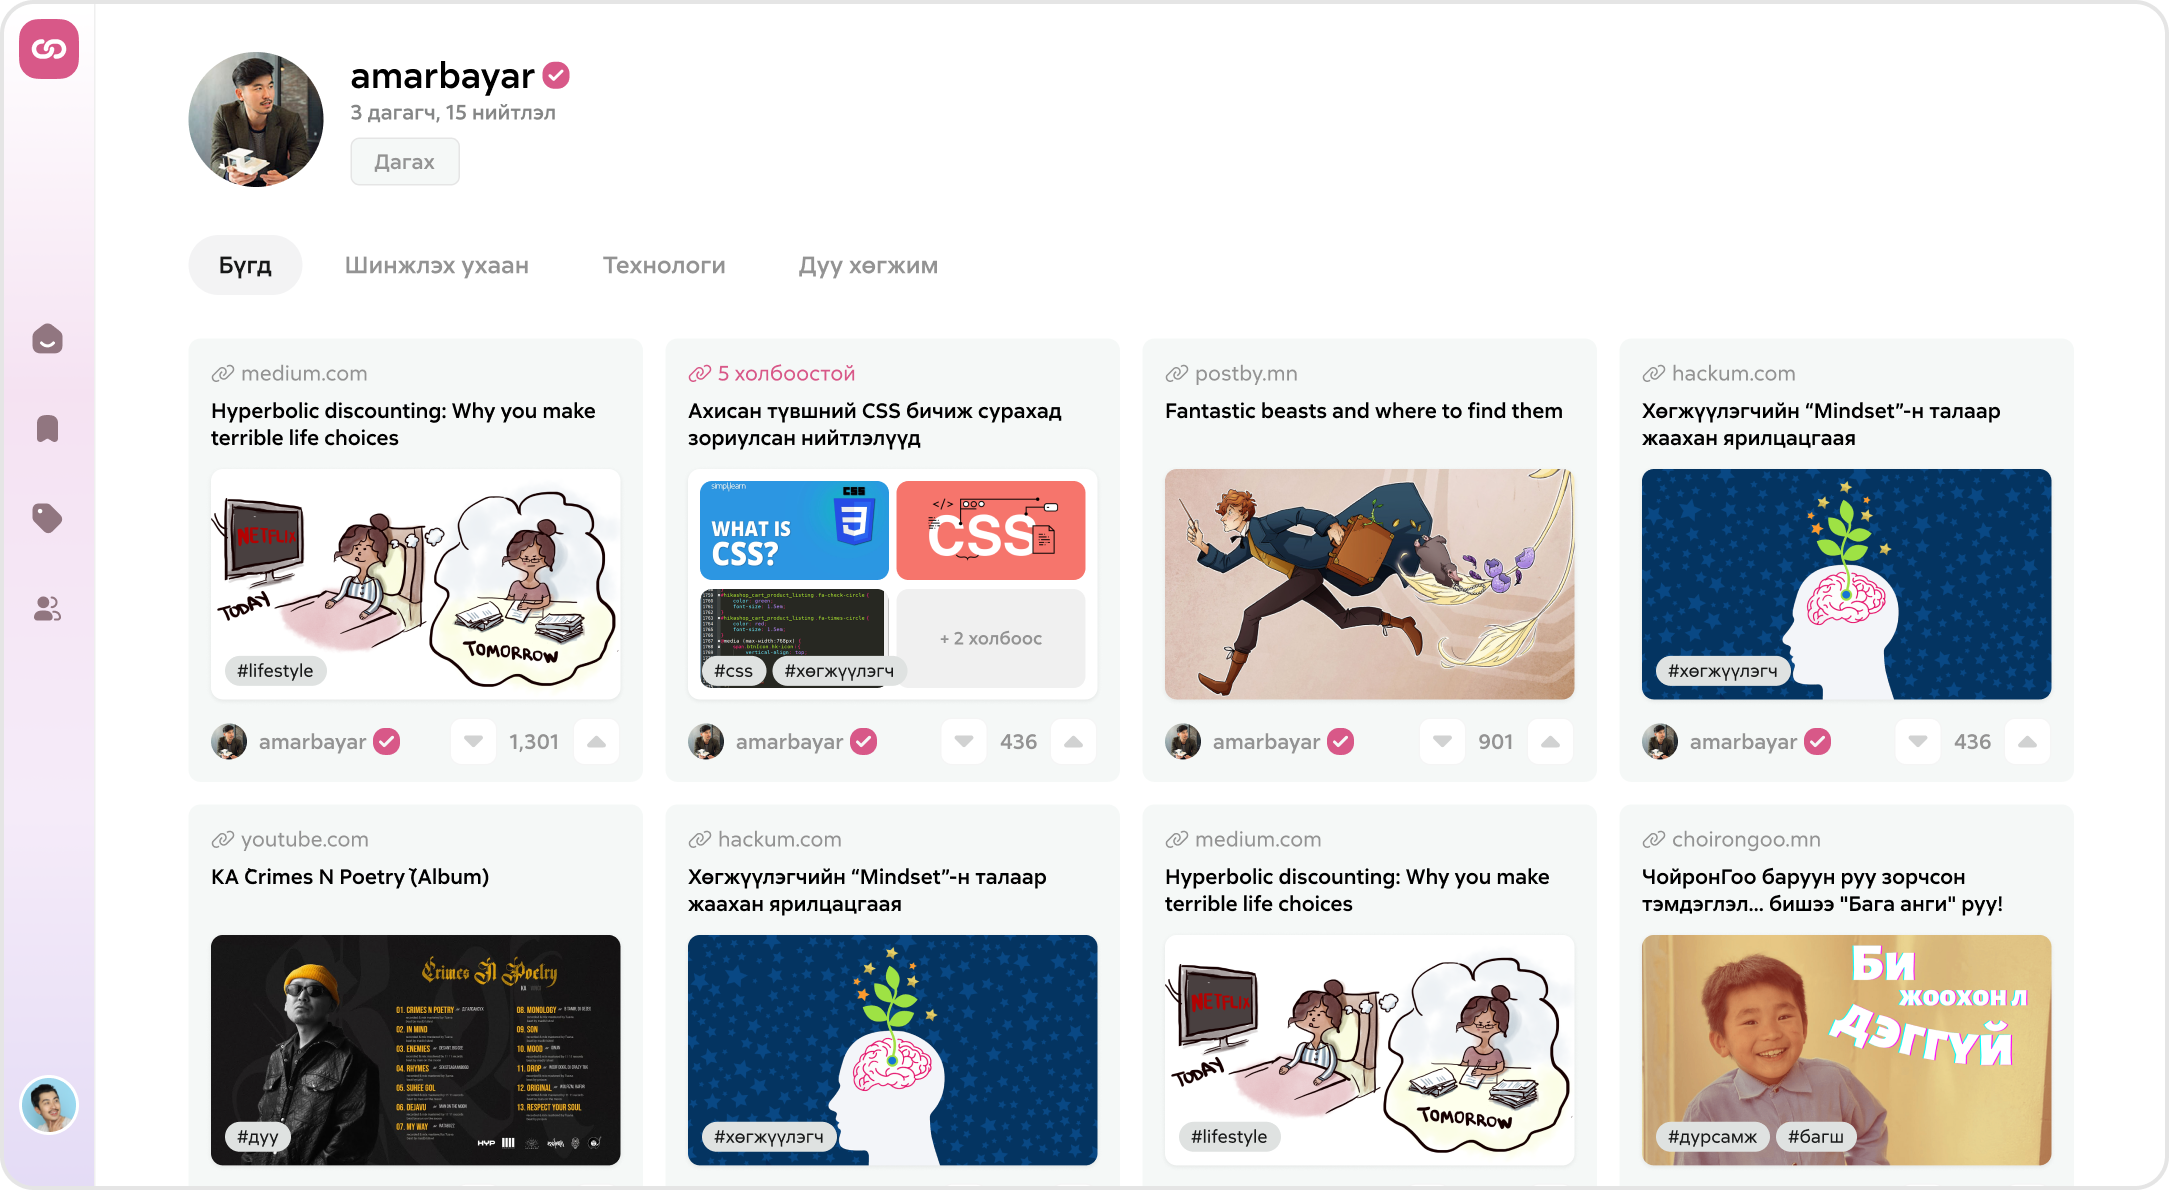
\includegraphics[width=10cm]{images/interfaces/profile.png}
% 	\caption{Бусдын профайлыг харах хуудас}
% 	\label{fig:profile}
% \end{figure}

% \begin{figure}[h]
% 	\centering
% 	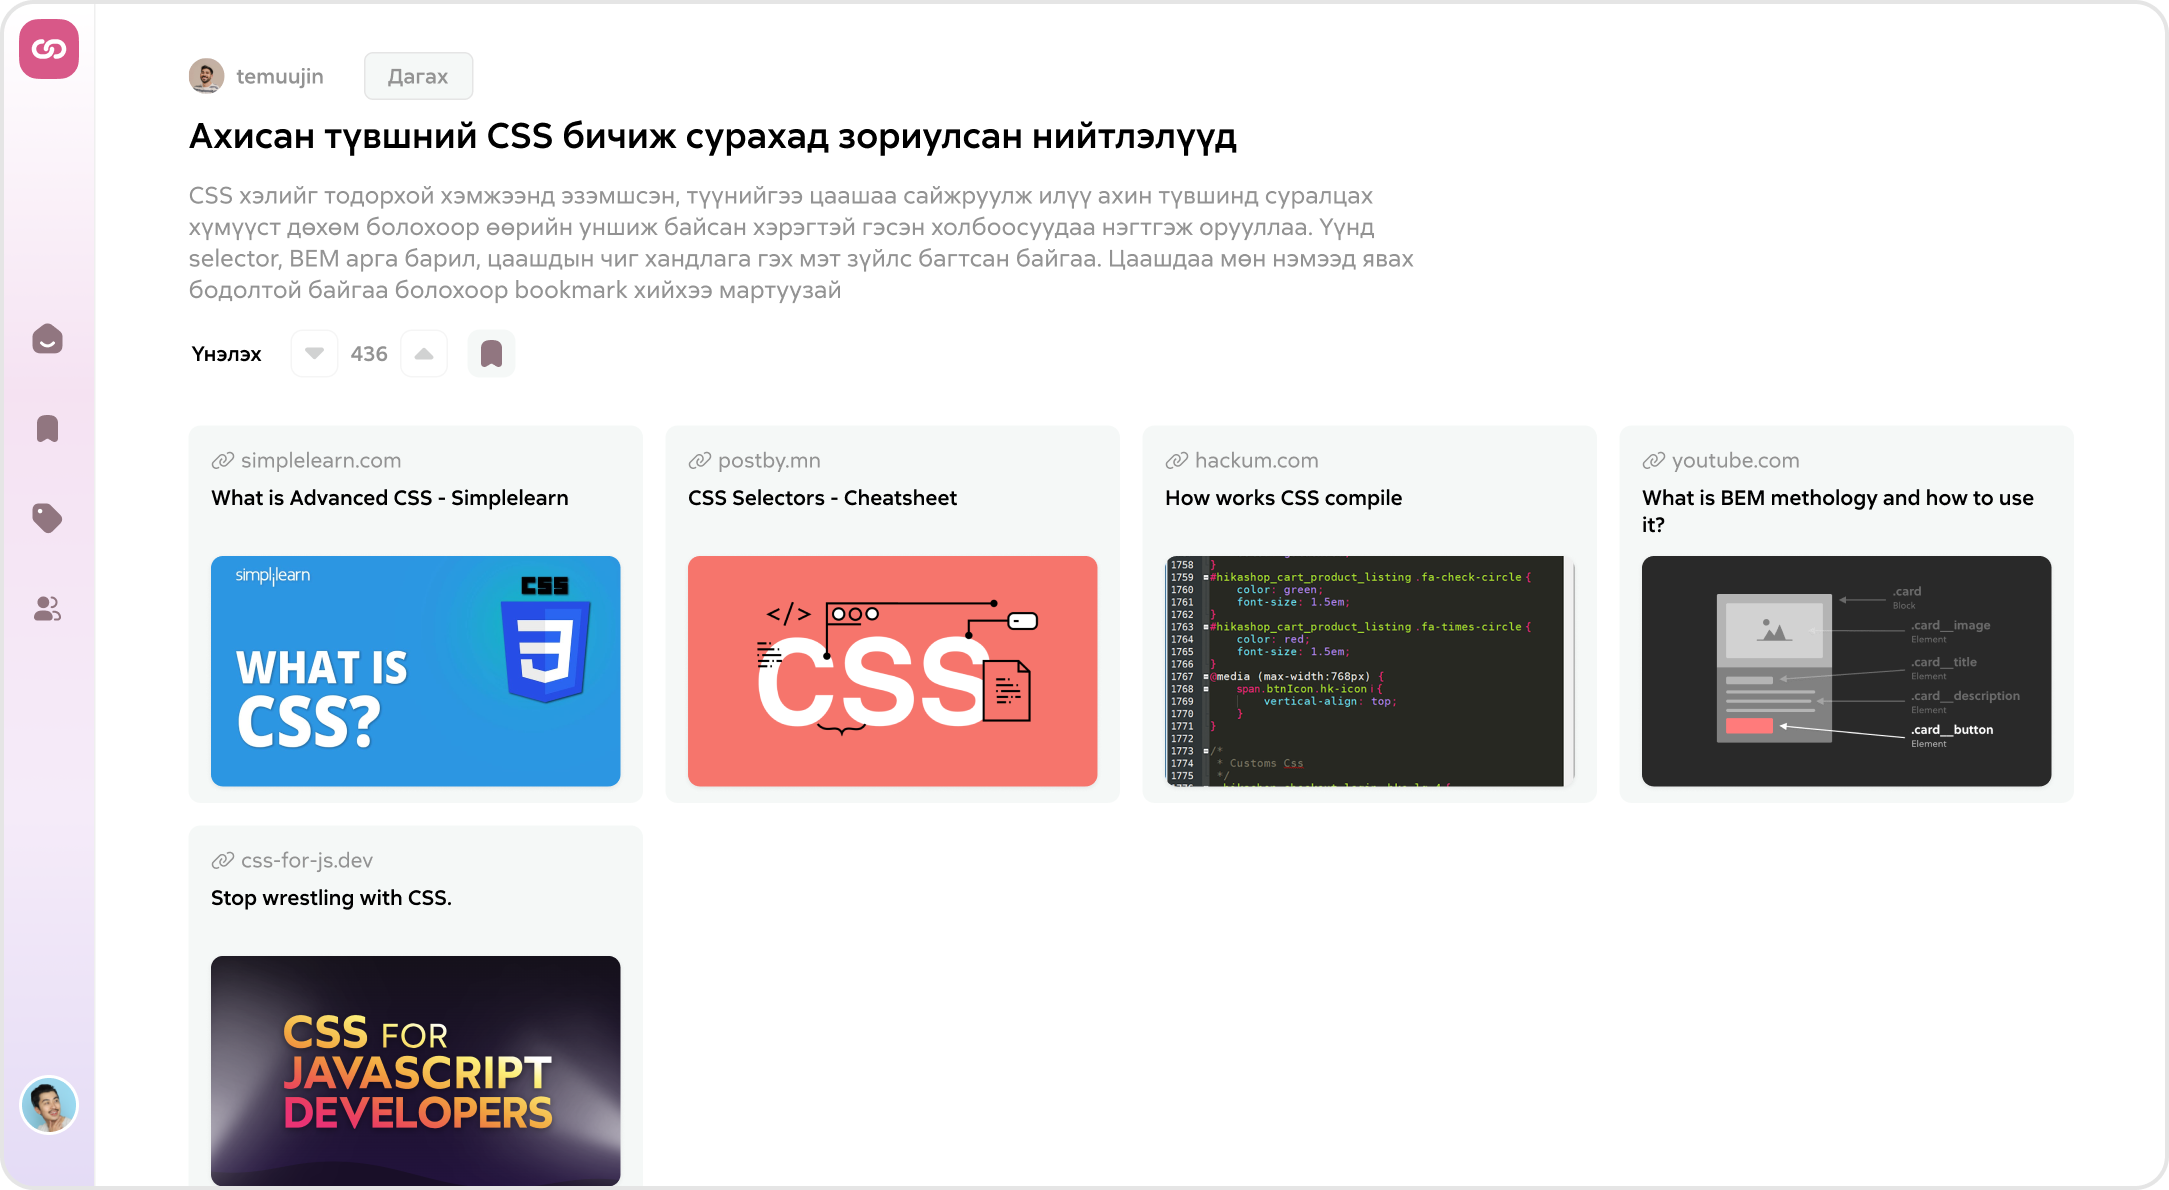
\includegraphics[width=10cm]{images/interfaces/grouped-link.png}
% 	\caption{Бүлэг холбоос доторх холбоосуудыг харах хуудас}
% 	\label{fig:grouped}
% \end{figure}

% \clearpage
% \section{Өгөгдлийн сан}

% \subsection{Өгөгдлийн сангийн диаграм}
% \begin{figure}[h]
% 	\centering
% 	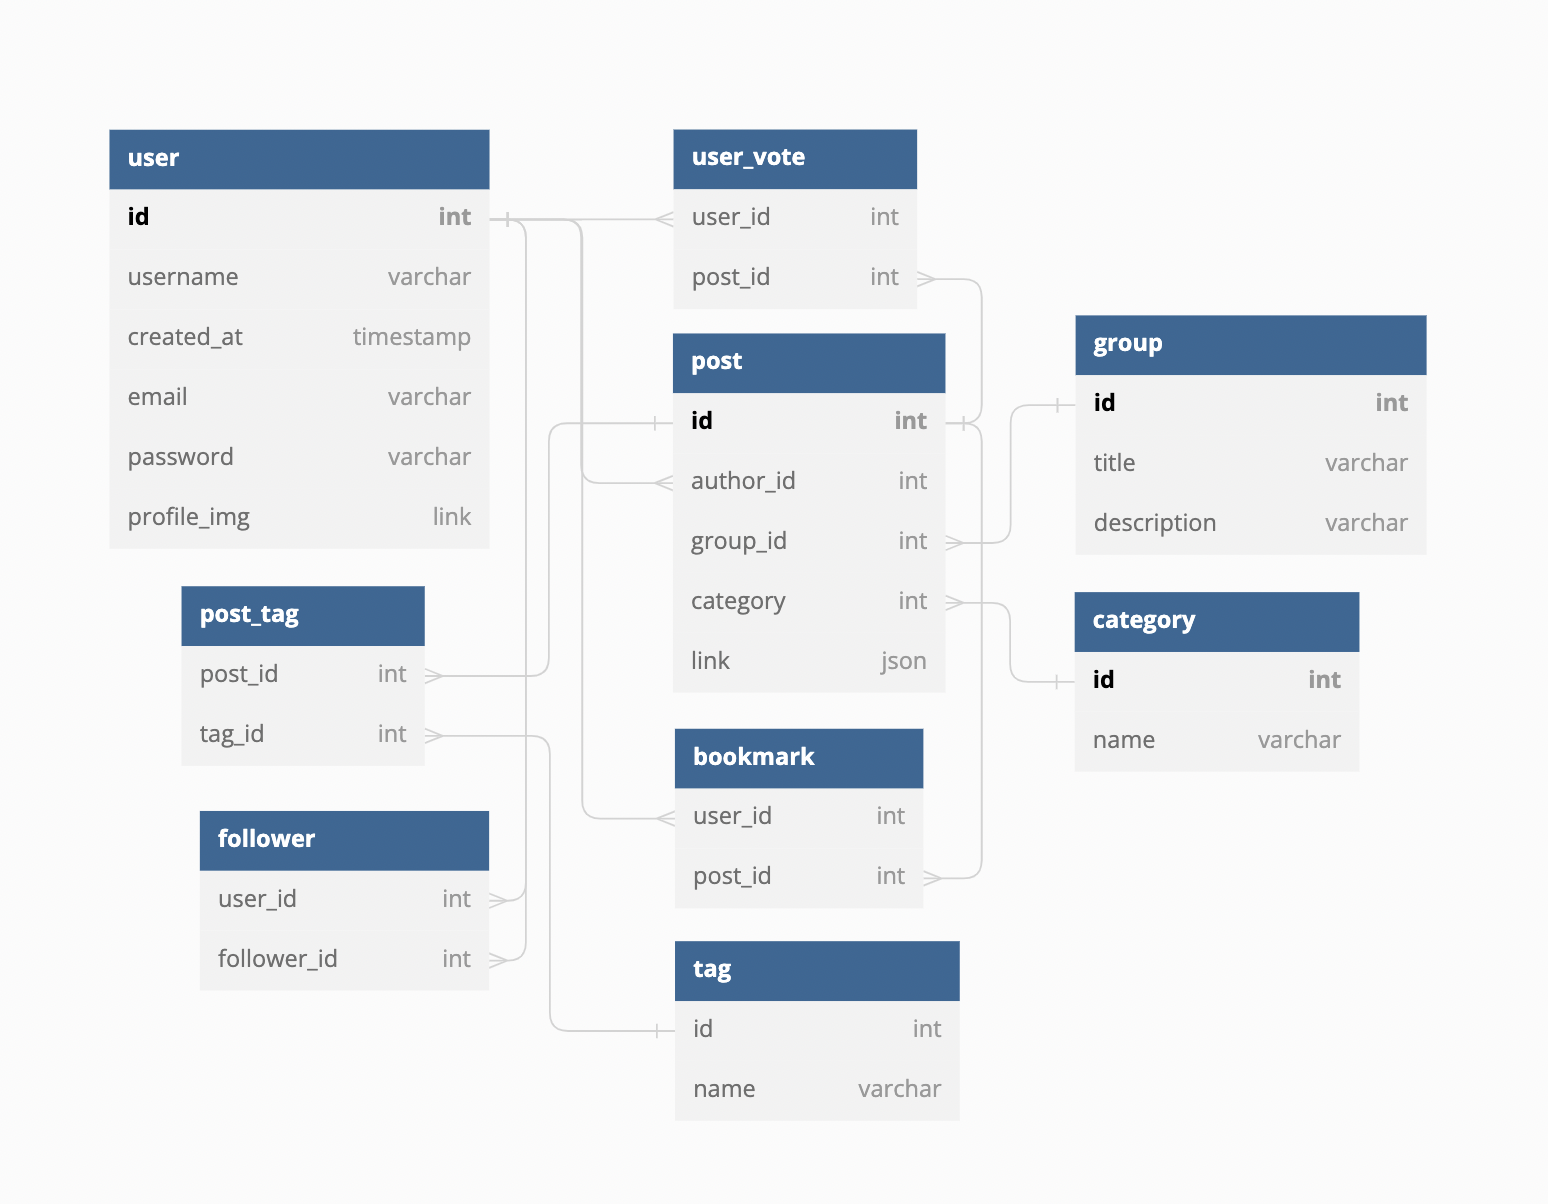
\includegraphics[width=15cm]{images/erdiagram.png}
% 	\caption{Системийн RD Schema}
% 	\label{fig:erd}
% \end{figure}

% \textbf{Өгөгдлийн сангийн хүснэгтүүдийн тайлбар}

% \begin{table}[h]
% 	\caption{user хүснэгт}
% 	\begin{tabular}{|l|l|l|p{8cm}|}
% 	\hline
% 	№ &  Талбарын нэр & Өгөгдлийн төрөл & Тайлбар \\ \hline
% 	1 &  id & int & Хэрэглэгчийн дахин давтагдашгүй ID-г хадгална - Auto Incremented \\ \hline
% 	2 &  username & varchar & Хэрэглэгчийн гараас оруулж өгсөн нэрийг хадгална. Зөвхөн латин тэмдэгтүүд ашиглах хэрэгтэй \\ \hline
% 	3 &  created\_at & timestamp & Хэрэглэгчийн хаяг үүссэн хугацааг серверээс авч хадгална \\ \hline
% 	4 &  email & varchar & Хэрэглэгчийн цахим шуудан \\ \hline
% 	5 &  password & varchar & Хэрэглэгчийн гараас оруулж өгсөн нууц үгийг encrypt-лэж уг хэсэгт хадгална \\ \hline
% 	6 &  profile\_img & link & Хэрэглэгчийн оруулж өгсөн зургийг сервер дээр хадгалж, замыг нь энэ хэсэгт хадгална \\ \hline

% \end{tabular}
% \end{table}

% \begin{table}[h]
% 	\caption{post хүснэгт}
% 	\begin{tabular}{|l|l|l|p{8cm}|}
% 	\hline
% 	№ &  Талбарын нэр & Өгөгдлийн төрөл & Тайлбар \\ \hline
% 	1 &  id & int & Нийтлэлийн дахин давтагдашгүй ID-г хадгална - Auto Incremented \\ \hline
% 	2 &  author\_id & int & Тухайн нийтлэлийг бичсэн хэрэглэгчийн ID-г Foreign Key-р хадгална \\ \hline
% 	3 &  group\_id & int & Хэрэглэгч веб холбоосыг нэг дор олныг оруулах боломжтой ба тухайн тохиолдолд бүлэг веб холбоос гэж үзэн тухайн бүлгийн нэр, тайлбарыг хадгална \\ \hline
% 	4 &  category & int & Нийтлэлийн төрлийг хадгална. Нийтлэл дор хаяж нэг нийтлэлд харьяалагдах шаардлагатай \\ \hline
% 	5 &  link & json & Нэг болон түүнээс их холбоос хадгалах боломжтой болгож байгаа тул хэрэглэгчийн оруулж өгсөн веб холбоосуудыг уг талбарт json хэлбэрээр хадгална \\ \hline

% \end{tabular}
% \end{table}

% \begin{table}[h]
% 	\caption{post\_tag хүснэгт}
% 	\begin{tabular}{|l|l|l|p{8cm}|}
% 	\hline
% 	№ &  Талбарын нэр & Өгөгдлийн төрөл & Тайлбар \\ \hline
% 	1 &  post\_id & int & Нэг нийтлэл хэдэн ч tag-тай байж болох ба уг талбарт нийтлэлийн ID-г Foreign Key-р авч ашиглаж байгаа \\ \hline
% 	2 &  tag\_id & int & Хэрэглэгч өөрсдөө Tag-аа үүсгэж өгөх боломжтой учир тухайн үүсгэсэн Tag-н ID-г авна \\ \hline

% \end{tabular}
% \end{table}

% \begin{table}[h]
% 	\caption{follower хүснэгт}
% 	\begin{tabular}{|l|l|l|p{8cm}|}
% 	\hline
% 	№ &  Талбарын нэр & Өгөгдлийн төрөл & Тайлбар \\ \hline
% 	1 &  user\_id & int & Тухайн хэрэглэгчид хэнийг дагаж байгааг илэрхийлэх талбар \\ \hline
% 	2 &  follower\_id & int & Тухайн хэрэглэгчийг хэн дагаж байгааг илэрхийлэх талбар \\ \hline

% \end{tabular}
% \end{table}

% \begin{table}[h]
% 	\caption{user\_vote хүснэгт}
% 	\begin{tabular}{|l|l|l|p{8cm}|}
% 	\hline
% 	№ &  Талбарын нэр & Өгөгдлийн төрөл & Тайлбар \\ \hline
% 	1 &  user\_id & int & Хэн тухайн нийтлэл дээр санал өгсныг хадгалах талбар \\ \hline
% 	2 &  post\_id & int & Тухайн хэрэглэгч аль нийтлэл дээр санал өгсныг хадгалах талбар \\ \hline

% \end{tabular}
% \end{table}

% \begin{table}[h]
% 	\caption{group хүснэгт}
% 	\begin{tabular}{|l|l|l|p{8cm}|}
% 	\hline
% 	№ &  Талбарын нэр & Өгөгдлийн төрөл & Тайлбар \\ \hline
% 	1 &  id & int & Primary Key бөгөөд хэрэглэгч олон веб холбоос оруулж өгөх боломжтой. Үүнийг бид бүлэг холбоос гэж нэрлэж байгаа ба энэ тохиолдолд тухайн бүлэгт заавал нэр болон тайлбар утга байх хэрэгтэй \\ \hline
% 	2 &  title & varchar & Бүлэг холбоосын гарчгийг хадгалах талбар \\ \hline
% 	3 &  description & varchar & Бүлэн холбоосын тайлбарыг хадгалах талбар \\ \hline

% \end{tabular}
% \end{table}

% \begin{table}[h]
% 	\caption{category хүснэгт}
% 	\begin{tabular}{|l|l|l|p{8cm}|}
% 	\hline
% 	№ &  Талбарын нэр & Өгөгдлийн төрөл & Тайлбар \\ \hline
% 	1 &  id & int & Primary Key бөгөөд хэрэглэгч нийтлэлийн төрөл олон байх боломжтой. \\ \hline
% 	2 &  name & varchar & Төрлийн нэрийг хадгалах талбар \\ \hline

% \end{tabular}
% \end{table}

% \begin{table}[h]
% 	\caption{bookmark хүснэгт}
% 	\begin{tabular}{|l|l|l|p{8cm}|}
% 	\hline
% 	№ &  Талбарын нэр & Өгөгдлийн төрөл & Тайлбар \\ \hline
% 	1 &  user\_id & int & Хэрэглэгч өөрт таалагдсан нийтлэлээ хадгалах шаардлагатай ба уг талбарт тухайн нийтлэлийг хадгалсан хэрэглэгчийн ID-г Foreign Key-р хадгална \\ \hline
% 	2 &  post\_id & int & Хэрэглэгчийн хадгалсан нийтлэлийн ID-г хадгална \\ \hline

% \end{tabular}
% \end{table}

% \begin{table}[h]
% 	\caption{tag хүснэгт}
% 	\begin{tabular}{|l|l|l|p{8cm}|}
% 	\hline
% 	№ &  Талбарын нэр & Өгөгдлийн төрөл & Тайлбар \\ \hline
% 	1 &  id & int & Хэрэглэгчийн гараас оруулж өгсөн tag-н ID-г хадгална - Auto Incremented \\ \hline
% 	2 &  name & int & Хэрэглэгчийн гараас оруулж өгсөн tag-н нэрийг уг талбарт хадгална \\ \hline

% \end{tabular}
% \end{table}


\clearpage





